\documentclass{scrartcl}
\usepackage{tabularx}
\usepackage{booktabs}
\usepackage{csquotes}
% Include Graphic-files:
\usepackage{graphicx}
\usepackage{caption}
\usepackage{subfig}
\usepackage{url}
%\usepackage{subfig}
\newsubfloat{figure}
\newcommand{\source}[1]{\vspace{-3pt} \caption*{ Source: {#1}} }

\begin{document}

\begin{figure}[!t]
\centering
  \begin{minipage}{0.23\textwidth}
  \centering
    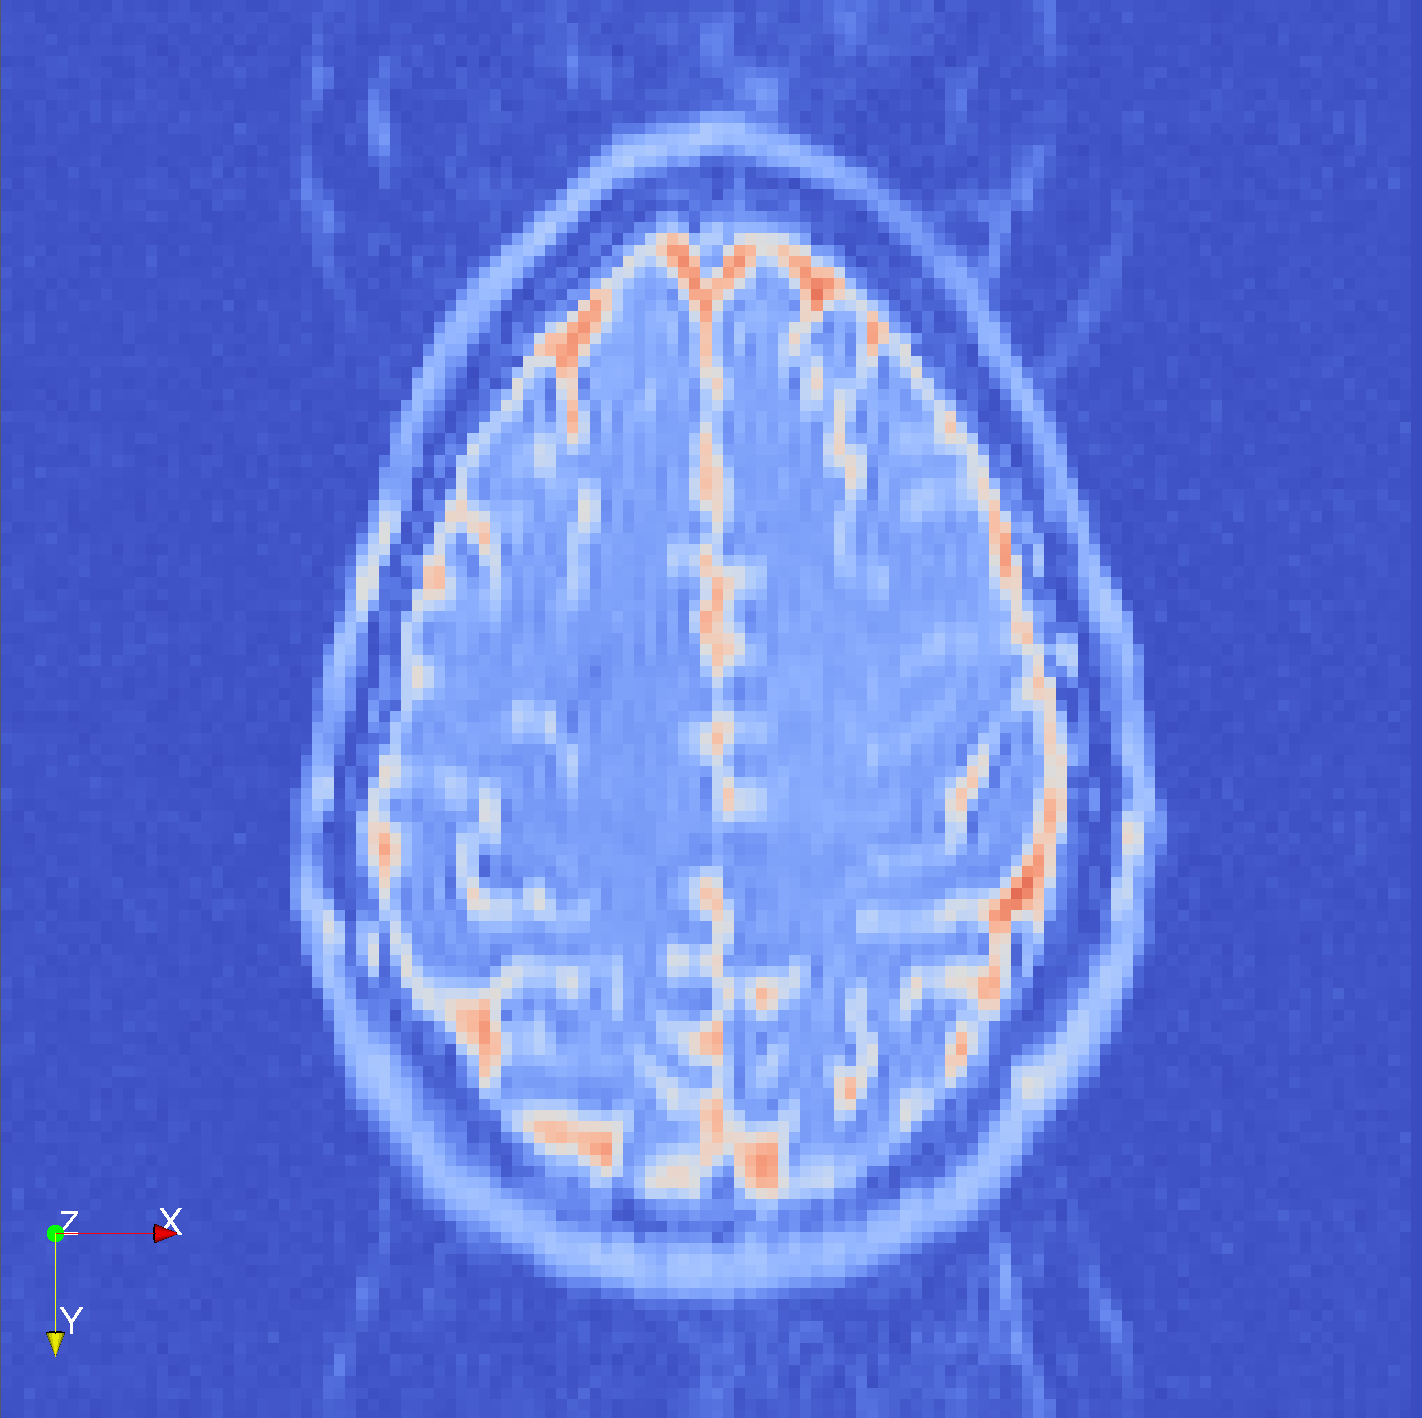
\includegraphics[width=\textwidth]{brain_org.png}
    \label{a)}
	a)
  \end{minipage}
  \begin{minipage}{0.23\textwidth}
  \centering
    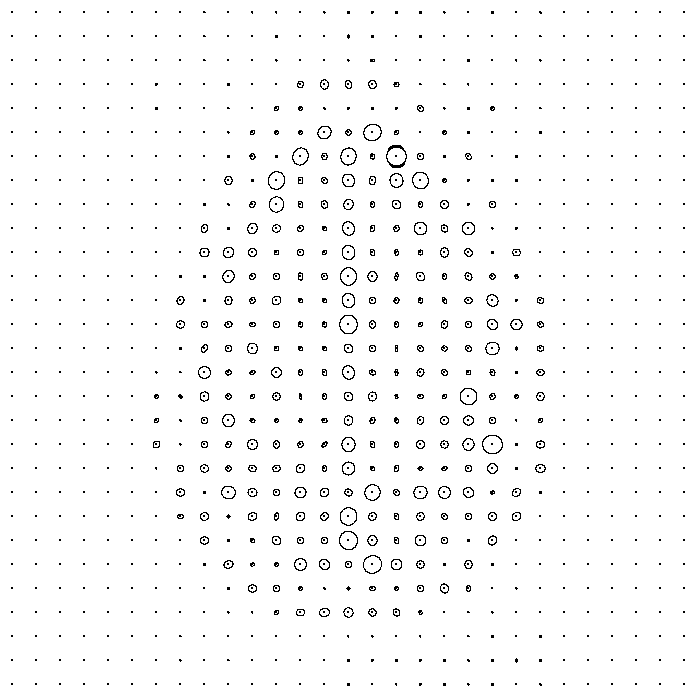
\includegraphics[width=\textwidth]{brainDwnsmpl.png}
    \label{b)}
    b)
  \end{minipage}
  \begin{minipage}{0.23\textwidth}
  \centering
    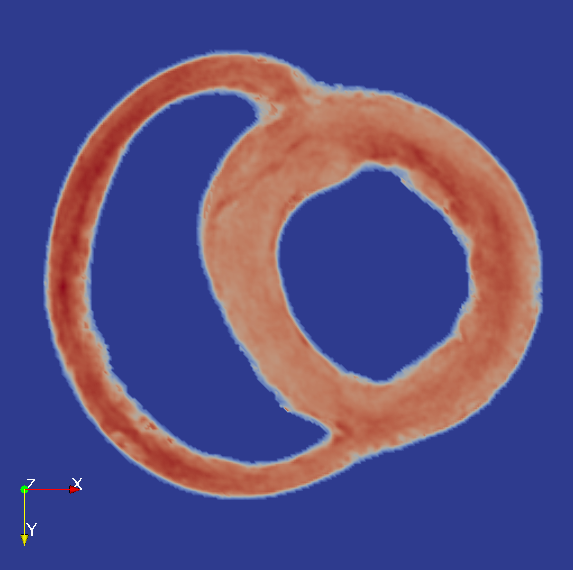
\includegraphics[width=\textwidth]{heart_org.png}
    \label{b)}
    a)
  \end{minipage}
  \begin{minipage}{0.23\textwidth}
  \centering
    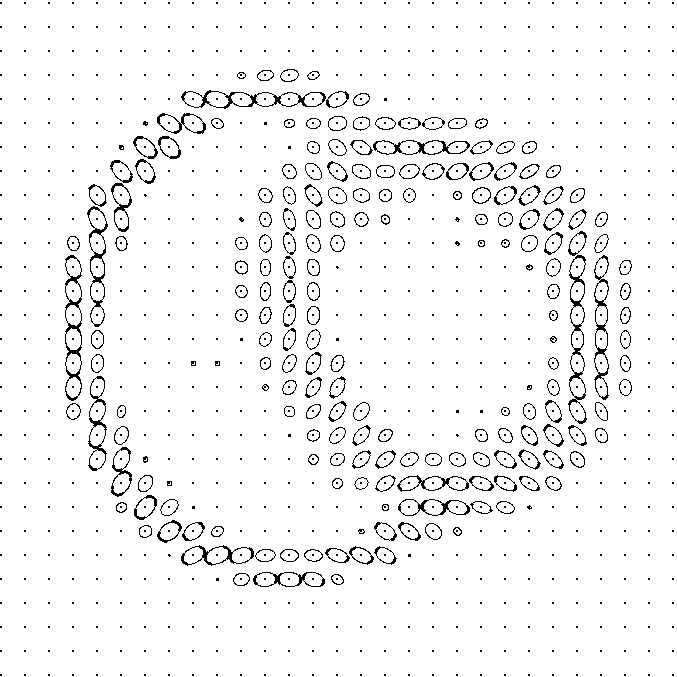
\includegraphics[width=\textwidth]{heartDwnsmpl.png}
    \label{b)}
    b)
  \end{minipage}
\caption{Brain and Heart dataset: a) tensor magnitude, b) ellipsoid glyphs}
\label{real1}
\end{figure}



%%%%%%%%%%%%%%%%%%%%%%%%%%%%%%%%%%%%%%%%%%%%%%%%%%%%%%%%%%%%

% Alternative: put content in separate files
% Check the difference between including these files using \input{filename} and \include{filename} and see which one you like better
%\chapter{Einleitung}\label{intro}
%\input{introduction}
%
%\chapter{Voraussetzungen}\label{bg}
%\input{background}



\end{document}